\documentclass[12pt,a4paper]{article}
\usepackage[utf8]{inputenc}
\usepackage{amsmath}
\usepackage{amsfonts}
\usepackage{amssymb}
\usepackage{graphicx}
\usepackage{tikz}
\usepackage{array}
\usepackage{geometry}
\usepackage{hyperref}
\geometry{a4paper, margin=1in}

\title{Regression Analysis by Example \\ (5th Edition)}
\author{Author: Chatterjee \\ \small A Complete Practical Guide for Engineers and Data Analysts}
\date{}

\begin{document}
	
	\maketitle
	
	\tableofcontents
	\newpage
	
	\section{Introduction}
	Regression analysis is one of the most powerful tools in modern engineering, statistics, data science, and predictive analytics. From predicting system failures in mechanical engineering to modeling financial markets, regression techniques allow engineers and analysts to understand relationships between variables and make data-driven decisions.
	
	The concept of regression analysis dates back to the 19th century when statisticians began studying relationships between biological traits and heredity. Today, regression models are widely used in fields such as:
	\begin{itemize}
		\item Civil engineering
		\item Electrical engineering
		\item Mechanical engineering
		\item Artificial intelligence
		\item Machine learning
		\item Economics
		\item Environmental science
		\item Healthcare analytics
	\end{itemize}
	
	The book “Regression Analysis by Example (5th Edition)” is considered one of the most practical references for learning regression. Instead of focusing only on theoretical mathematics, it teaches regression through real-world examples, making the concept easier to understand for beginners while still offering depth for professionals.
	
	\section{Background Theory}
	Before diving into regression techniques, it’s important to understand the statistical foundations behind them.
	
	\subsection{Relationship Between Variables}
	In engineering and science, we often want to understand how one variable affects another.
	
	Example relationships include:
	
	\begin{table}[h!]
		\centering
		\begin{tabular}{|c|c|c|}
			\hline
			\textbf{Independent Variable} & \textbf{Dependent Variable} & \textbf{Example} \\
			\hline
			Temperature & Material Expansion & Thermal engineering \\
			Voltage & Current & Electrical circuits \\
			Pressure & Flow Rate & Fluid mechanics \\
			Advertising Budget & Sales & Business analytics \\
			\hline
		\end{tabular}
		\caption{Variable Relationships}
	\end{table}
	
	Regression analysis helps determine how strong this relationship is and allows us to create mathematical models describing it.
	
	\subsection{Correlation vs Regression}
	Many beginners confuse correlation with regression.
	
	\begin{table}[h!]
		\centering
		\begin{tabular}{|c|c|}
			\hline
			\textbf{Concept} & \textbf{Purpose} \\
			\hline
			Correlation & Measures strength of relationship \\
			Regression & Creates predictive mathematical model \\
			\hline
		\end{tabular}
	\end{table}
	
	Correlation answers: \textit{“Are these variables related?”}
	
	Regression answers: \textit{“How can we predict one variable from another?”}
	
	\subsection{Statistical Foundations}
	Regression analysis relies on several statistical concepts:
	\begin{itemize}
		\item \textbf{Mean (Average)}:
		\[
		\bar{x} = \frac{\sum x_i}{n}
		\]
		\item \textbf{Variance}: Measures how spread out data points are.
		\item \textbf{Standard Deviation}: Indicates how far values deviate from the average.
		\item \textbf{Covariance}: Shows how two variables change together.
	\end{itemize}
	
	\subsection{Scatter Plot Visualization}
	A scatter plot helps visualize relationships between variables.
	
	\begin{center}
		\begin{tikzpicture}
			\draw[->] (0,0) -- (5,0) node[right] {$x$};
			\draw[->] (0,0) -- (0,5) node[above] {$y$};
			\filldraw (1,1) circle (2pt);
			\filldraw (2,2) circle (2pt);
			\filldraw (3,3) circle (2pt);
			\filldraw (4,4) circle (2pt);
			\filldraw (4.5,4.5) circle (2pt);
		\end{tikzpicture}
	\end{center}
	
	If the points form a pattern or line, regression modeling becomes possible.
	
	\section{Technical Definition}
	Regression analysis is a statistical method used to estimate the relationship between a dependent variable and one or more independent variables.
	
	Mathematically, regression models describe relationships using equations.
	
	\subsection{Basic Linear Regression Equation}
	\[
	Y = a + bX + \epsilon
	\]
	Where:
	\begin{table}[h!]
		\centering
		\begin{tabular}{|c|c|}
			\hline
			\textbf{Symbol} & \textbf{Meaning} \\
			\hline
			$Y$ & Dependent variable \\
			$X$ & Independent variable \\
			$a$ & Intercept \\
			$b$ & Slope \\
			$\epsilon$ & Error term \\
			\hline
		\end{tabular}
	\end{table}
	
	\subsection{Meaning of the Slope ($b$)}
	The slope indicates how much $Y$ changes when $X$ increases by one unit.\\
	Example: If $b = 2$, then every increase of 1 unit in $X$ increases $Y$ by 2 units.
	
	\subsection{Intercept ($a$)}
	The intercept is the value of $Y$ when $X = 0$. In engineering models, the intercept often represents:
	\begin{itemize}
		\item Initial conditions
		\item Baseline system output
		\item Default measurement level
	\end{itemize}
	
	\section{Step-by-Step Explanation of Regression Analysis}
	Understanding regression becomes easier when broken down into systematic steps.
	
	\subsection{Step 1: Collect Data}
	Data collection is the foundation of regression modeling.
	
	Example dataset:
	\begin{table}[h!]
		\centering
		\begin{tabular}{|c|c|}
			\hline
			\textbf{Temperature (°C)} & \textbf{Expansion (mm)} \\
			\hline
			20 & 2.1 \\
			30 & 3.2 \\
			40 & 4.5 \\
			50 & 5.1 \\
			60 & 6.4 \\
			\hline
		\end{tabular}
	\end{table}
	
	\subsection{Step 2: Plot the Data}
	Plotting helps visually inspect relationships.
	
	\begin{center}
		\begin{tikzpicture}
			\draw[->] (0,0) -- (5,0) node[right] {Temperature};
			\draw[->] (0,0) -- (0,5) node[above] {Expansion};
			\filldraw (1,1) circle (2pt);
			\filldraw (2,1.5) circle (2pt);
			\filldraw (3,2.5) circle (2pt);
			\filldraw (4,3) circle (2pt);
			\filldraw (5,4) circle (2pt);
		\end{tikzpicture}
	\end{center}
	
	The upward trend indicates positive correlation.
	
	\subsection{Step 3: Calculate Regression Coefficients}
	Using formulas:
	\[
	b = \frac{\sum (x - \bar{x})(y - \bar{y})}{\sum (x - \bar{x})^2}
	\]
	\[
	a = \bar{y} - b\bar{x}
	\]
	
	These equations calculate the best fitting line.
	
	\subsection{Step 4: Construct the Regression Model}
	Example result:
	\[
	Y = 0.8 + 0.095X
	\]
	Meaning:
	\begin{itemize}
		\item Intercept = 0.8
		\item Expansion increases 0.095 mm per degree Celsius
	\end{itemize}
	
	\subsection{Step 5: Evaluate the Model}
	Several metrics are used.
	
	\subsubsection{Coefficient of Determination ($R^2$)}
	\[
	R^2 = 0.92
	\]
	This means 92\% of the variation is explained by the model.
	
	\subsection{Step 6: Validate the Model}
	Validation ensures the regression model is reliable.
	
	Methods include:
	\begin{itemize}
		\item Residual analysis
		\item Cross-validation
		\item Statistical significance tests
	\end{itemize}
	
	\section{Comparison of Regression Types}
	Regression is not limited to linear relationships.
	
	\subsection{Common Types of Regression}
	\begin{table}[h!]
		\centering
		\begin{tabular}{|c|c|c|}
			\hline
			\textbf{Type} & \textbf{Description} & \textbf{Use Case} \\
			\hline
			Linear Regression & Straight-line relationship & Engineering measurements \\
			Multiple Regression & Multiple variables & System modeling \\
			Polynomial Regression & Curved relationship & Physics simulations \\
			Logistic Regression & Binary outcome & Medical diagnosis \\
			Ridge Regression & Handles multicollinearity & Machine learning \\
			Lasso Regression & Feature selection & AI modeling \\
			\hline
		\end{tabular}
	\end{table}
	
	\subsection{Linear vs Multiple Regression}
	\begin{table}[h!]
		\centering
		\begin{tabular}{|c|c|c|}
			\hline
			\textbf{Feature} & \textbf{Linear Regression} & \textbf{Multiple Regression} \\
			\hline
			Variables & 1 independent variable & Multiple variables \\
			Complexity & Simple & Moderate \\
			Example & Temperature vs expansion & Temperature + pressure vs expansion \\
			\hline
		\end{tabular}
	\end{table}
	
	\section{Diagrams and Tables}
	
	\subsection{Regression Line Illustration}
	\begin{center}
		\begin{tikzpicture}
			\draw[->] (0,0) -- (5,0) node[right] {$x$};
			\draw[->] (0,0) -- (0,5) node[above] {$y$};
			\draw[blue, thick] (0,0.5) -- (5,4.5) node[midway, above] {Regression Line};
			\filldraw (1,1) circle (2pt);
			\filldraw (2,2.5) circle (2pt);
			\filldraw (3,3) circle (2pt);
			\filldraw (4,4) circle (2pt);
		\end{tikzpicture}
	\end{center}
	
	\subsection{Residual Error Diagram}
	Residual = difference between actual and predicted value.
	
	\begin{center}
		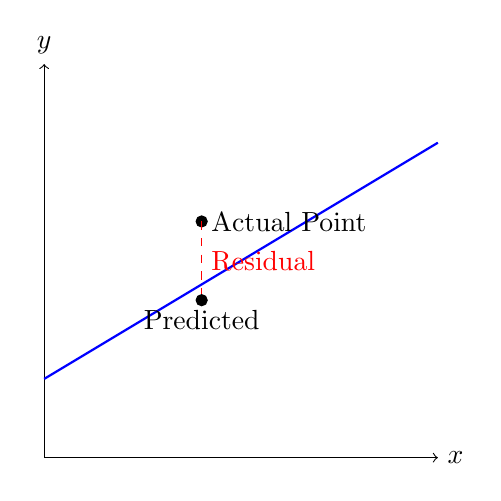
\begin{tikzpicture}
			\draw[->] (0,0) -- (5,0) node[right] {$x$};
			\draw[->] (0,0) -- (0,5) node[above] {$y$};
			\draw[blue, thick] (0,1) -- (5,4);
			\filldraw (2,3) circle (2pt) node[right] {Actual Point};
			\draw[dashed, red] (2,3) -- (2,2) node[midway, right] {Residual};
			\filldraw (2,2) circle (2pt) node[below] {Predicted};
		\end{tikzpicture}
	\end{center}
	
	Residual analysis helps evaluate model accuracy.
	
	\subsection{Table: Residual Example}
	\begin{table}[h!]
		\centering
		\begin{tabular}{|c|c|c|c|}
			\hline
			$X$ & Actual $Y$ & Predicted $Y$ & Residual \\
			\hline
			10 & 15 & 14 & 1 \\
			20 & 25 & 24 & 1 \\
			30 & 33 & 35 & -2 \\
			\hline
		\end{tabular}
	\end{table}
	
	\section{Examples of Regression Analysis}
	
	\subsection{Example 1: Electrical Engineering}
	Predict current using voltage. Ohm's law relationship:
	\[
	I = \frac{V}{R}
	\]
	Regression can estimate resistance using measured data.
	
	\subsection{Example 2: Civil Engineering}
	Predict bridge stress based on load.
	\begin{table}[h!]
		\centering
		\begin{tabular}{|c|c|}
			\hline
			\textbf{Load (tons)} & \textbf{Stress (MPa)} \\
			\hline
			10 & 3 \\
			20 & 5 \\
			30 & 7 \\
			\hline
		\end{tabular}
	\end{table}
	Regression predicts stress for larger loads.
	
	\subsection{Example 3: Mechanical Engineering}
	Predict machine wear over time.
	\begin{table}[h!]
		\centering
		\begin{tabular}{|c|c|}
			\hline
			\textbf{Operating Hours} & \textbf{Wear Level} \\
			\hline
			100 & 0.5 \\
			200 & 1.1 \\
			300 & 1.6 \\
			\hline
		\end{tabular}
	\end{table}
	Regression allows prediction of maintenance schedules.
	
	\section{Real World Applications}
	Regression analysis is used in many engineering industries.
	
	\subsection{Civil Engineering}
	Applications include:
	\begin{itemize}
		\item Traffic flow prediction
		\item Structural load analysis
		\item Construction cost estimation
	\end{itemize}
	Example: Predicting bridge lifespan using environmental factors.
	
	\subsection{Electrical Engineering}
	Regression helps in:
	\begin{itemize}
		\item Power consumption forecasting
		\item Signal processing
		\item Circuit modeling
	\end{itemize}
	Example: Predicting battery life based on usage patterns.
	
	\subsection{Artificial Intelligence}
	Regression models are foundational for machine learning. Applications include:
	\begin{itemize}
		\item Price prediction
		\item Demand forecasting
		\item Fraud detection
	\end{itemize}
	
	\subsection{Automotive Engineering}
	Used for:
	\begin{itemize}
		\item Fuel consumption modeling
		\item Engine performance prediction
		\item Autonomous vehicle algorithms
	\end{itemize}
	
	\subsection{Environmental Engineering}
	Regression helps analyze:
	\begin{itemize}
		\item Air pollution trends
		\item Climate modeling
		\item Water quality prediction
	\end{itemize}
	
	\section{Common Mistakes in Regression Analysis}
	Even experienced engineers sometimes make regression mistakes.
	
	\subsection{Ignoring Outliers}
	Outliers distort regression models.
	\begin{center}
		\begin{tikzpicture}
			\draw[->] (0,0) -- (5,0);
			\draw[->] (0,0) -- (0,5);
			\filldraw (1,1) circle (2pt);
			\filldraw (2,2) circle (2pt);
			\filldraw (3,3) circle (2pt);
			\filldraw (4,4) circle (2pt);
			\filldraw (4.5,1) circle (2pt) node[right] {Outlier};
		\end{tikzpicture}
	\end{center}
	Solution: Detect using box plots, use robust regression methods.
	
	\subsection{Assuming Causation}
	Regression shows correlation, not causation. Example: Ice cream sales and drowning rates both increase in summer. Regression shows correlation but not cause.
	
	\subsection{Overfitting the Model}
	Too many variables can cause overfitting. The model fits the training data perfectly but fails on new data.
	
	\subsection{Ignoring Residual Analysis}
	Residuals must be randomly distributed. Patterns indicate a poor model.
	
	\subsection{Multicollinearity}
	Occurs when independent variables are highly correlated. Example: Temperature and humidity both affecting energy consumption.
	
	\section{Challenges \& Solutions}
	Regression modeling involves practical challenges.
	
	\subsection{Challenge 1: Missing Data}
	Real-world datasets often contain missing values.\\
	\textbf{Solution:} Imputation, Data interpolation, Removing incomplete records.
	
	\subsection{Challenge 2: Nonlinear Relationships}
	Some systems behave nonlinearly.\\
	\textbf{Solution:} Polynomial regression, Logarithmic transformation.
	
	\subsection{Challenge 3: High Dimensional Data}
	Large datasets with many variables can complicate analysis.\\
	\textbf{Solution:} Principal Component Analysis (PCA), Feature selection.
	
	\subsection{Challenge 4: Noise in Data}
	Sensors and measurement devices introduce noise.\\
	\textbf{Solution:} Data filtering, Smoothing techniques.
	
	\section{Case Study: Predicting Energy Consumption}
	
	\subsection{Problem}
	A power company wants to predict electricity demand based on temperature.
	
	\subsection{Data}
	\begin{table}[h!]
		\centering
		\begin{tabular}{|c|c|}
			\hline
			\textbf{Temperature (°C)} & \textbf{Energy Use (MW)} \\
			\hline
			15 & 320 \\
			20 & 350 \\
			25 & 390 \\
			30 & 450 \\
			35 & 520 \\
			\hline
		\end{tabular}
	\end{table}
	
	\subsection{Regression Model}
	Result:
	\[
	\text{Energy} = 180 + 10.2 \times \text{Temperature}
	\]
	
	\subsection{Interpretation}
	For every 1°C increase, energy demand increases by 10.2 MW.
	
	\subsection{Impact}
	The company uses the model to:
	\begin{itemize}
		\item Predict power demand
		\item Optimize electricity production
		\item Avoid blackouts
	\end{itemize}
	
	\section{Tips for Engineers Using Regression}
	\begin{enumerate}
		\item \textbf{Always Visualize Data First:} Scatter plots reveal relationships before modeling.
		\item \textbf{Use Statistical Software:} Common tools include Python, R, MATLAB, Excel, SPSS.
		\item \textbf{Validate Models with New Data:} Always test models using unseen datasets.
		\item \textbf{Understand Assumptions:} Linear regression assumes linear relationship, normal error distribution, constant variance.
		\item \textbf{Combine Domain Knowledge with Statistics:} Engineering knowledge improves model accuracy.
	\end{enumerate}
	
	\section{Frequently Asked Questions (FAQs)}
	
	\begin{enumerate}
		\item \textbf{What is regression analysis used for?} \\
		Regression analysis predicts relationships between variables and is widely used in engineering, finance, and data science.
		
		\item \textbf{What is the difference between regression and correlation?} \\
		Correlation measures relationship strength, while regression builds predictive mathematical models.
		
		\item \textbf{What does $R^2$ mean?} \\
		$R^2$ represents how much of the variation in the dependent variable is explained by the regression model.
		
		\item \textbf{When should multiple regression be used?} \\
		Multiple regression is used when a system depends on more than one variable.
		
		\item \textbf{Is regression used in machine learning?} \\
		Yes. Regression is a fundamental technique in machine learning algorithms.
		
		\item \textbf{Can regression predict the future?} \\
		Regression can forecast trends based on historical data but cannot guarantee exact future outcomes.
		
		\item \textbf{What software is best for regression analysis?} \\
		Popular tools include Python, R, MATLAB, and Excel.
	\end{enumerate}
	
	\section{Conclusion}
	Regression analysis is one of the most valuable tools for engineers, scientists, and data analysts. By modeling relationships between variables, regression allows professionals to:
	\begin{itemize}
		\item Predict outcomes
		\item Optimize systems
		\item Identify trends
		\item Improve decision-making
	\end{itemize}
	
	The approach presented in \textit{Regression Analysis by Example (5th Edition)} emphasizes practical learning through real-world scenarios, making it an ideal resource for both beginners and advanced practitioners.
	
	As engineering fields increasingly rely on data-driven decision making, mastering regression analysis has become a crucial skill for modern professionals.
	
	Whether predicting structural loads, optimizing energy consumption, or building machine learning models, regression analysis remains a cornerstone of modern engineering and analytics.
	
\end{document}